\documentclass[a4paper,11pt]{article}

\usepackage[T1]{fontenc}
\usepackage[active]{srcltx}
\usepackage[english]{babel}
\usepackage[numbers]{natbib}
\usepackage[utf8]{inputenc}
\usepackage{amsmath}
\usepackage{amssymb}
%\usepackage{fullpage}
\usepackage{graphicx}
\usepackage{listings}
\usepackage{parskip}
\usepackage{srcltx}
\usepackage{url}

\urlstyle{same}

\newcommand{\m}[1]{\boldsymbol{#1}}
\renewcommand{\*}[0]{\cdot}
\renewcommand{\Pr}[1]{\mathbf{Pr}[#1]}
\renewcommand{\v}[1]{\vec{#1}}
\newcommand{\trans}[2][eng.]{(#1 \emph{#2})}

\title{
    {\sc DD2380 Artificial intelligence} \\
    Project report from group PIMP
}
\author{
    Joel Bohman \\ 881117 \and
    Samuel Lidén Borell \\ 881230 \and
    Joel Pettersson \\ 880519 \and
    Linus Wallgren \\ 880213
}
\date{\today}

\begin{document}
\maketitle
\thispagestyle{empty}
\newpage
\begin{abstract}
    % TODO write abstract
\end{abstract}
\thispagestyle{empty}
%\mbox{}
%\thispagestyle{empty}
\newpage
\setcounter{page}{1}


\part*{Introduction and background}

% - Some kind of introduction and one or two paragraphs about current solvers.
% - Short introduction to the problem and a description of the relationship to
%   the course material. also present what you think are your biggest
%   contributions so that this is clear. be sure to credit anyone that you got
%   help/code from

Sokoban is a puzzle created in 1981 by Hiroyuki Imabayashi. Sokoban is a
difficult puzzle and it has been proven that it is
PSPACE-complete~\cite{culberson1997}, which is a superset of NP. Current
solvers use techniques such as Iterative Deepening Search (IDS), Depth First
Search (DFS), Breadth-First Search (BFS), A* and combination of them to
traverse the search tree. Sokoban has a large branching factor which result in
a large search tree. To be able to traverse the search tree in any reasonable
time, pruning techniques and heuristics are necessary.  Humans can solve
Sokoban puzzles by advanced heuristics that becomes natural to us after playing
the game for a while.  


\section{Problem statement}

% a clear formalization of the problem using course material: which methods, how and why

Our task is to implement a program that is able to solve as many Sokoban levels
as possible. We have received test data that contains 136 levels to test our
solver against. However, we are not supposed to specialize our solver(s) for
this set of levels.


\part*{Theory and method}

% Explain the solutions we tried, answer why, how and what?
% A summary of your design approach and implementation

Sokoban can be solved by many different methods, as it is NP-hard and
PSPACE-complete it has not been proven that there exists an optimal solution,
but there are ways to prune the search tree and different kinds of heuristics
that can be used to find a solution faster. Our focus has been on pruning
techniques to reduce the size of the search tree, with heuristics for choosing
the search depth and solver. Our work resulted in three different solvers ---
IDSPusher, IDSPuller and a Bidirectional search combining them both.


\section{Solvers}

We chose to use iterative deepening search, also called IDS, when
implementing the solvers. The reason we chose IDS over breadth-first search,
BFS,  was simple, memory consumption. A normal BFS would need to store every
state it intends to visit in a queue, which would require large memory
footprint. Our original assumption was that depth-first search, DFS, would go
down too deep into the tree and possibly go past solutions, which was the
reason we originally chose IDS. IDS is simply a DFS that only goes down to a
certain level in the tree, if we find the solution we are done, otherwise we
increase the depth and try again.

When we began to implement the bidirectional search we found that IDS was
perfect, as we could simply let the agents take turn going deeper.

\subsection{IDSPusher}

To push the boxes around is the most natural solution, as it is how the game
actually works. The basic idea was a brute-force approach that mimicked the
human way to solve Sokoban puzzles. The naïve implementation of a pusher is
simple and easy to understand, however it is not particularly effective.
Because of this we implemented a couple of pruning techniques, like tunnel
detection and deadlock detection, which will be described later.

\subsection{IDSPuller}

Puller is our name for a method in which we reverse the goal and box positions.
Instead of trying to push boxes from their start positions to their goal we try
to pull boxes from the goals to their start positions. The advantage of this
approach is that no so called freeze deadlocks can occur~\cite{takes2007},
which reduces the number of useless state. This works because freeze deadlocks
occur when a box gets blocked by other boxes, and this can't happen when
pulling boxes because the player must be able to reach the square where the box
is to be pulled to.  It's still possible however to move a box such that some
boxes can no longer be reached.


\subsection{Bidirectional search using IDSPusher and IDSPuller}

Bidirectional search is a powerful way to reduce the search tree a lot
search~\cite{russell2009}. Instead of letting one solver go all the way we let
two solvers take turn to solve the board from both ends. As the size of the
search tree is exponential there is a lot to gain from this approach. Let's
look at an example.

% TODO: xun, ser detta ok ut?
In a complete binary tree, there is $2^n$ nodes on the level at depth $n$. Thus,
the total number of nodes is $2^n + 2^{(n-1)} + \ldots + 2^0$. Thinking of this
as a binary number we see that $2^n > 2^{(n-1)} + \ldots + 2^0$, e.g. $1000_2 =
8_{10} > 0111_2 = 7_{10}$. This implies that more than half of our nodes are on
the lowest level. When we use bidirectional search we only need to search to
half the depth --- two times. This means the number of nodes in the lowest level
will be $2^(n/2)$ for each one of the two solvers, which is much less than the
$2^n$ nodes required originally.

In a Sokoban problem the branch factor will typically be much higher than two
because there are often at least a couple of boxes that can be pushed from four
sides in the worst case (if there are no walls or other boxes at the sides).
That makes it even more efficient for this kind of search, even though pruning
techniques may reduce the average branch factor.



\section{Pruning techniques}

\subsection{Repeated states}

One of the probably most important pruning strategy is to check for repeated
states. We might arrive at a state following different paths in the search tree,
and exploring a node is only necessary to do once. That is, if we reach a state
that we recognize, it is time to stop following that road. In order not to be
required to store the whole board in a transposition table for repeated states
checking, we have chosen to use a hashing algorithm called Zobrist keys. In
addition to reducing memory usage, this type of hashing also allows constant
time comparison of boards.


\subsubsection{Zobrist keys}

\subsection{Deadlock}

\subsubsection{Dead squares deadlock}

\subsubsection{Freeze deadlock}

\subsection{No influence pushes --- tunnels}

\section{Heuristics}

\subsection{Lower bound}

\subsection{Choosing solver}


\part*{Results}


\part*{Discussion}

\section{Further improvements}

\subsection{A* and search heuristics}

\subsection{Corrals}

\subsection{Incremental reachable square search}

\part*{Conclusion}





Test \cite{culberson1997}.

Testing \cite{russell2009}.

Testing \cite{takes2007}.

\begin{figure}[h]
    \begin{center}
        \includegraphics{figures/equalState1}
        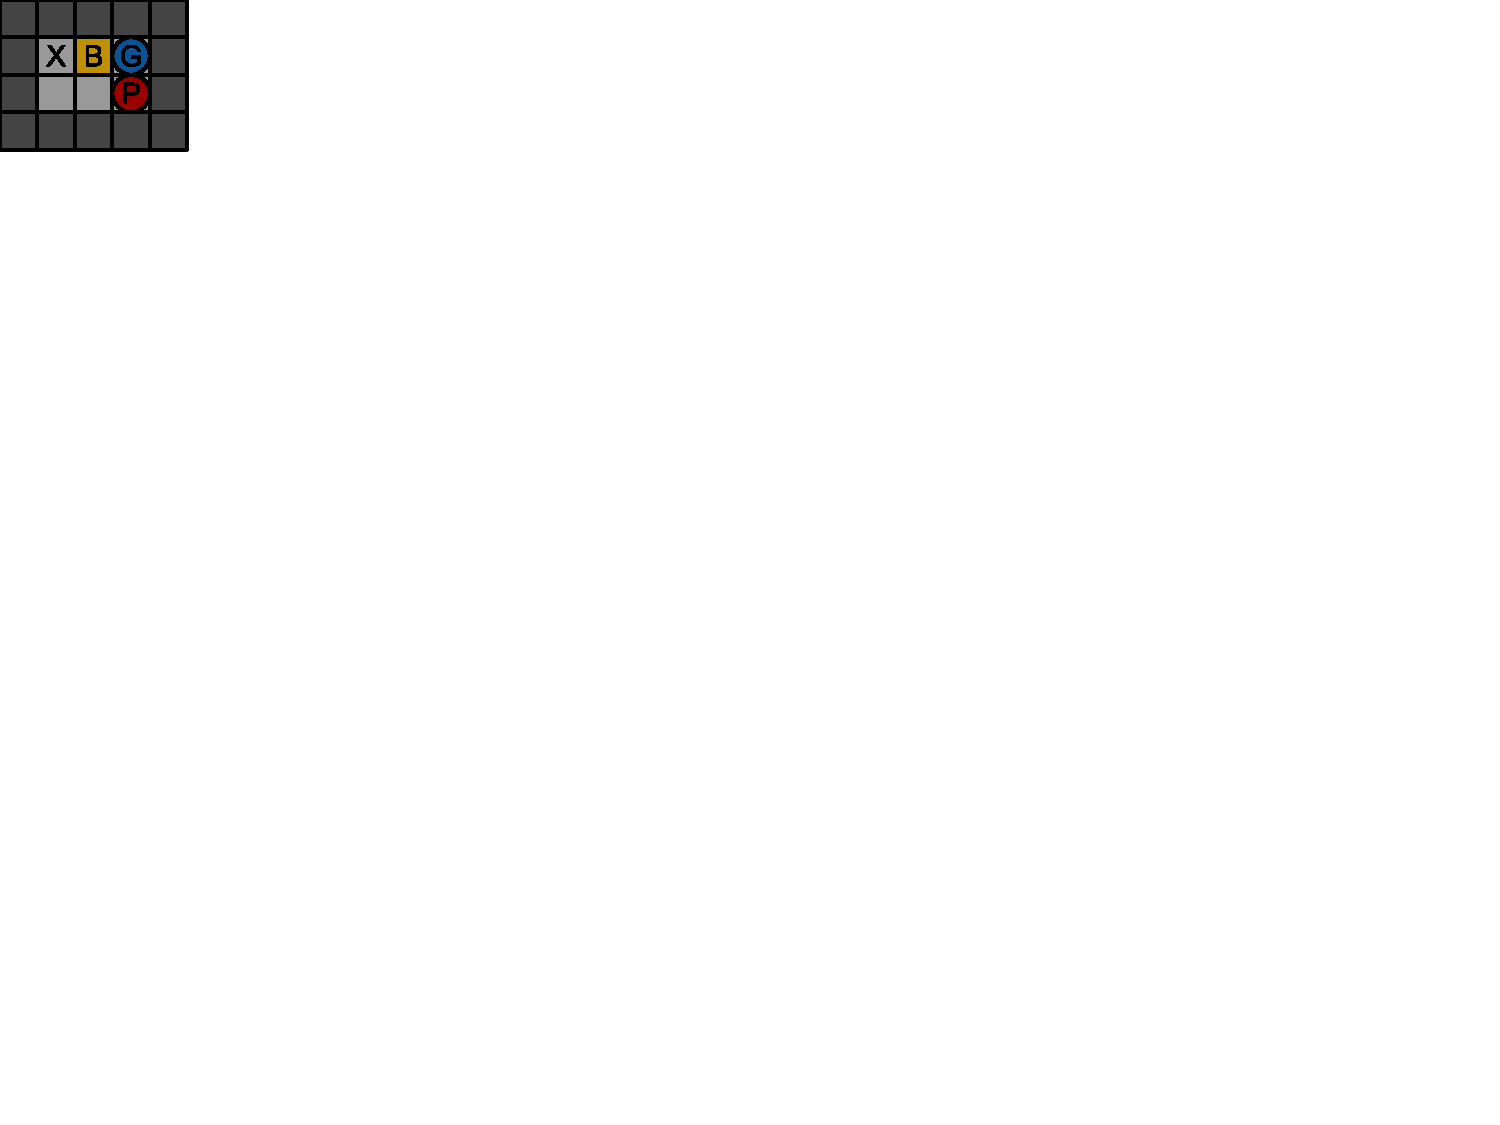
\includegraphics{figures/equalState2}
    \end{center}
    \caption{Test}
    \label{fig:test}
\end{figure}


\bibliographystyle{plainnat}
\bibliography{references} 


\end{document}
